\section{Launch The Simulation}

\begin{frame}[fragile]
	\frametitle{Launch Simulation Environment}
	In order to launch the simulation environment a ROS launch file is provided. Do the following command:
\begin{lstlisting}[language=bash]
$ roslaunch turtlebot3_autorace_simulation gazebo.launch
\end{lstlisting}

This launch file could take five input arguments:
\begin{itemize}
	\item \texttt{x\_pos}: set the x start coordinate of the robot
	\item \texttt{y\_pos}: set the y start coordinate of the robot
	\item \texttt{z\_pos}: set the z start coordinate of the robot
	\item \texttt{track}: set the track to import in the environment
	\item \texttt{use\_gui}: set if it has to load the user interface
\end{itemize}
By default it set $x = 0, y = 0, z = 0$, it set the track as \texttt{track1} and \texttt{use\_gui=True}
\end{frame}

\begin{frame}[fragile]
\frametitle{Launch Simulation Environment II}
Here is an example on how to launch the simulation with a different track:
\begin{lstlisting}[language=bash]
$ roslaunch turtlebot3_autorace_simulation gazebo.launch track:=track2
\end{lstlisting}
\begin{figure}
	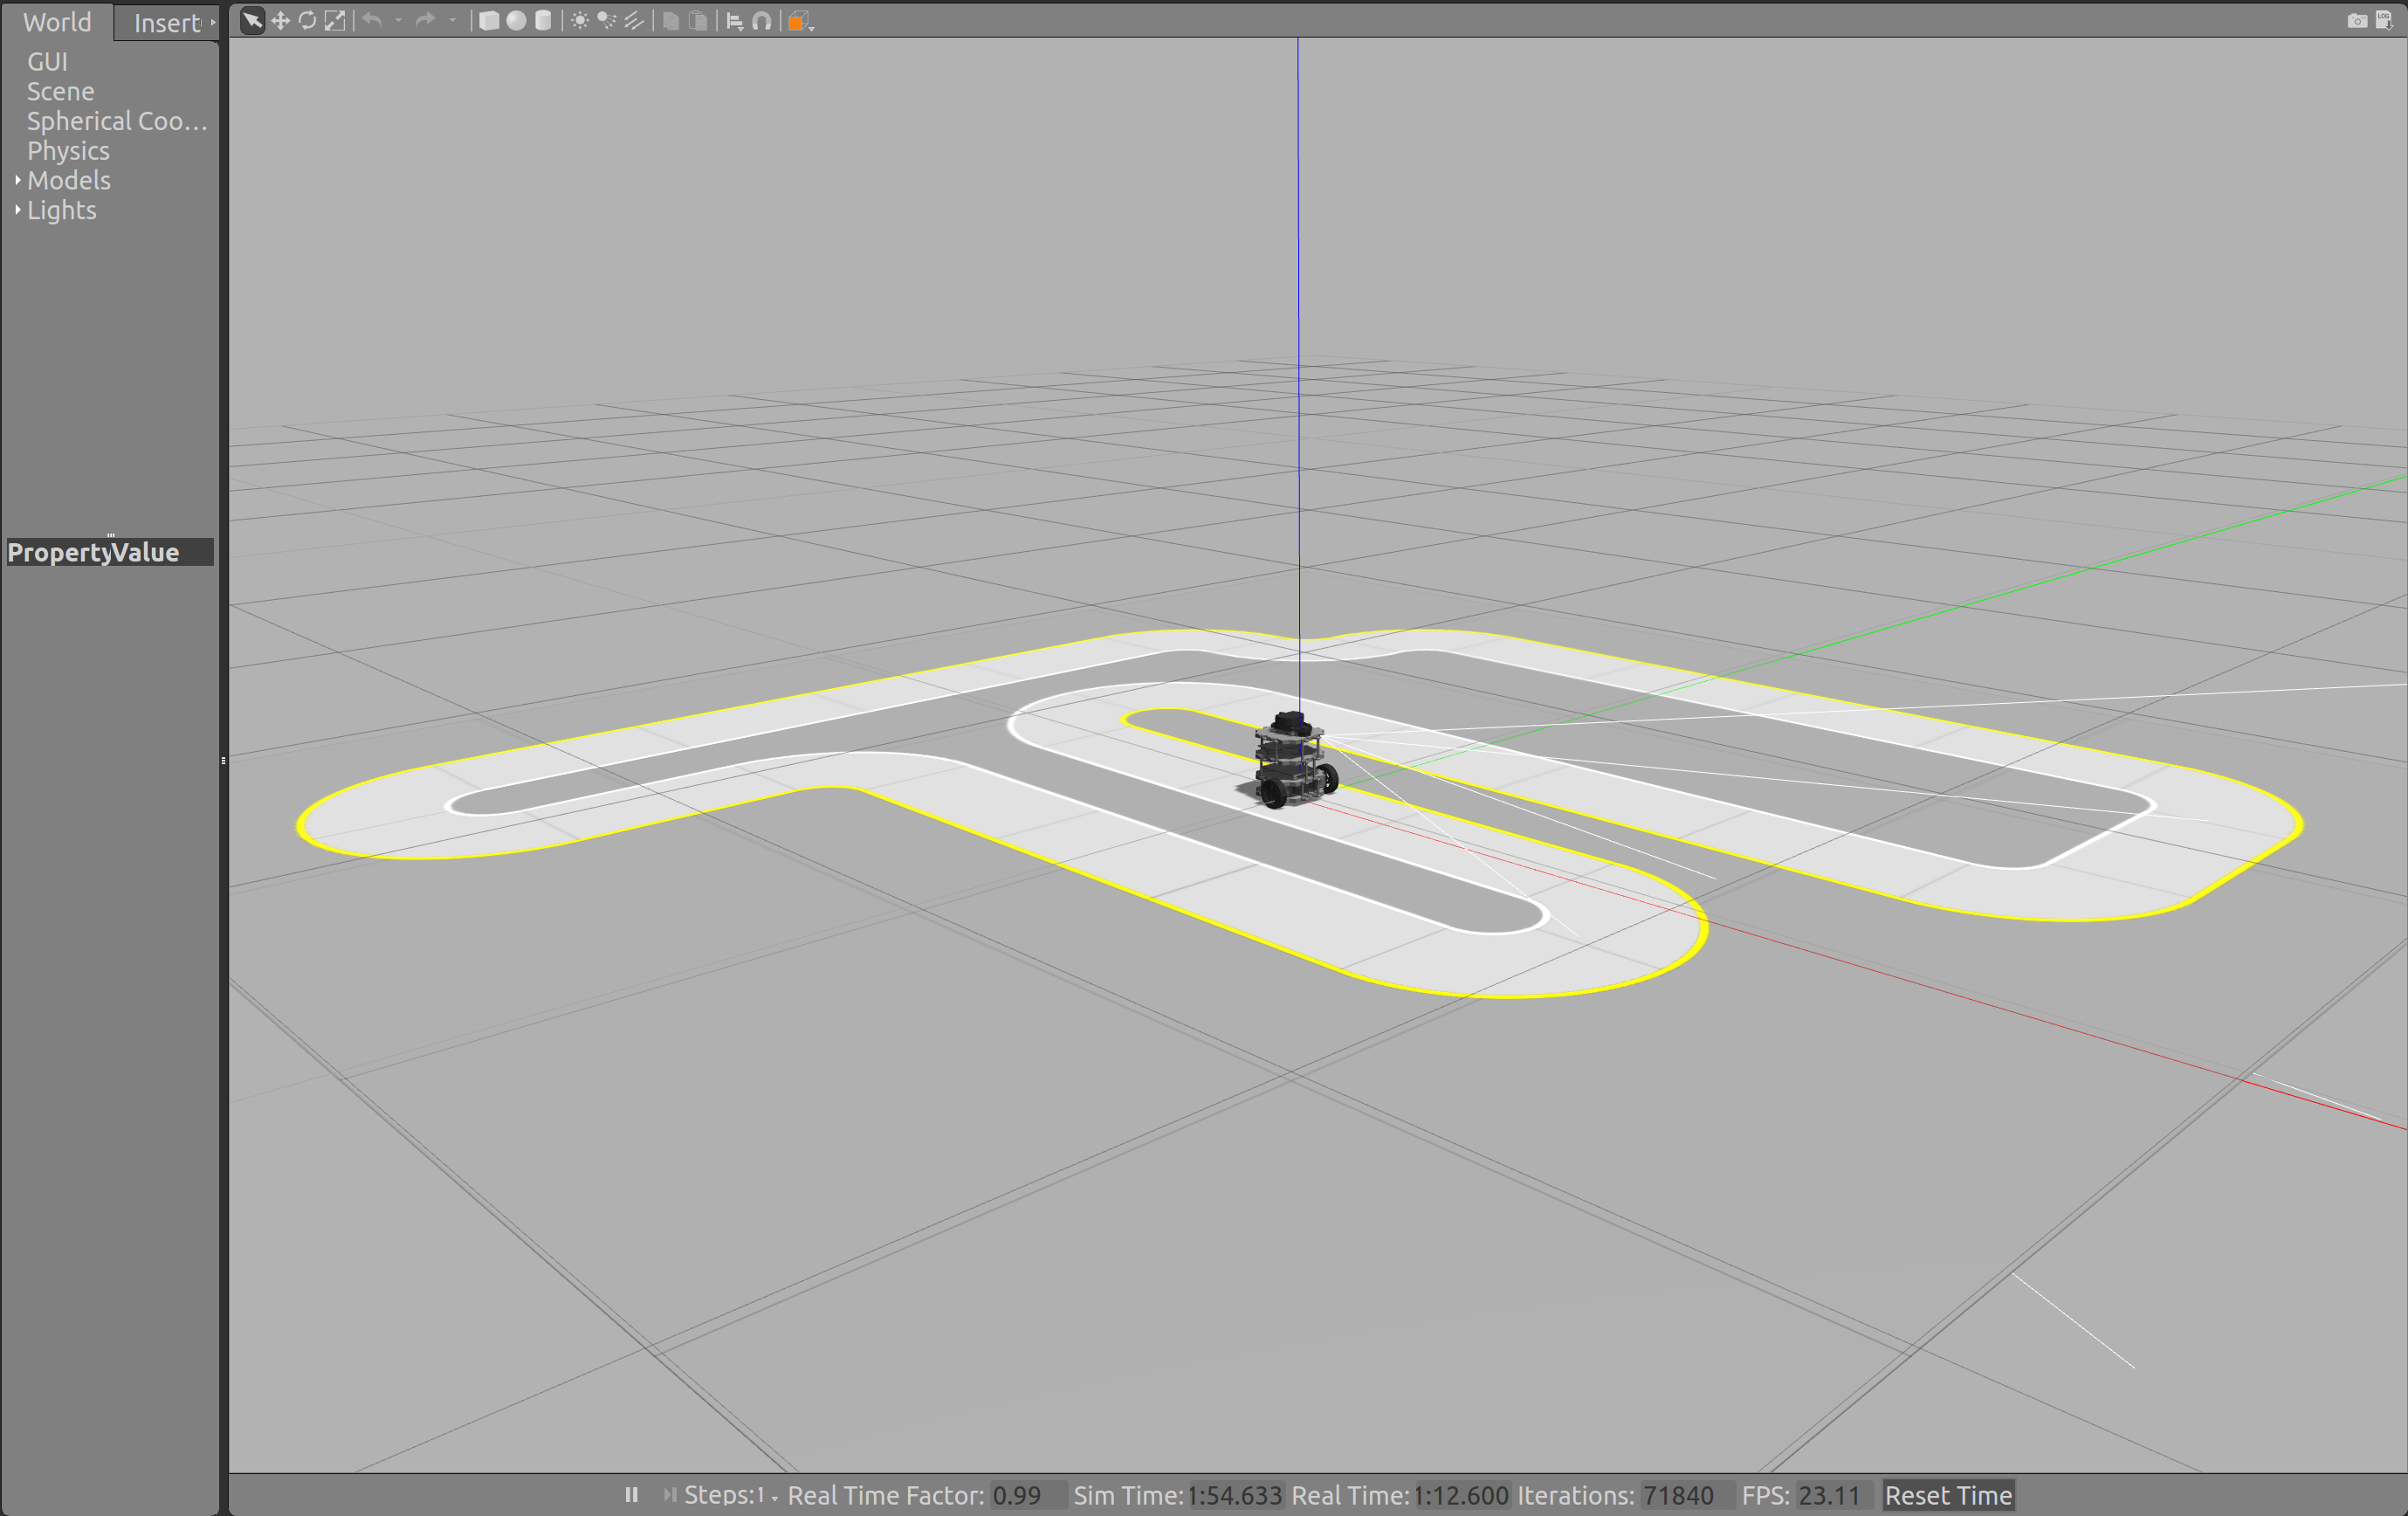
\includegraphics[width=0.7\textwidth]{figures/png/gazebo}
\end{figure}
\end{frame}

\begin{frame}[fragile]
	\frametitle{Launch Autodrive Nodes}
	In order to launch the Autodrive nodes a ROS launch file is provided. Do the following command:
\begin{lstlisting}[language=bash]
$ roslaunch turtlebot3_autorace_simulation autorace.launch
\end{lstlisting}

The calibration mode could be enabled by running the following command:
\begin{lstlisting}[language=bash]
$ roslaunch turtlebot3_autorace_simulation autorace.launch calibration_mode:=calibration
\end{lstlisting}
\end{frame}

\begin{frame}[fragile]
	\frametitle{Robot Visualization}
	In order to watch the image published on the ROS topics, a ROS launch file is provided. This launch file open \textit{RViz} and show the robot odometry and the images published on \texttt{/camera/rgb/image\_raw} and \texttt{/detect/lane}.
	
	To run \textit{RViz} do the following command:
\begin{lstlisting}
$ roslaunch turtlebot3_autorace_simulation rviz.launch
\end{lstlisting}
\end{frame}

\begin{frame}[fragile]
	\frametitle{Robot Visualization II}
	If your PC cannot execute \texttt{Gazebo} and \textit{RViz} simultaneously you should try to launch \texttt{Gazebo} with the \texttt{use\_gui} parameter setted to false:
\begin{lstlisting}[language=bash]
$ roslaunch turtlebot3_autorace_simulation gazebo.launch use_gui:=false
\end{lstlisting}
\begin{figure}
	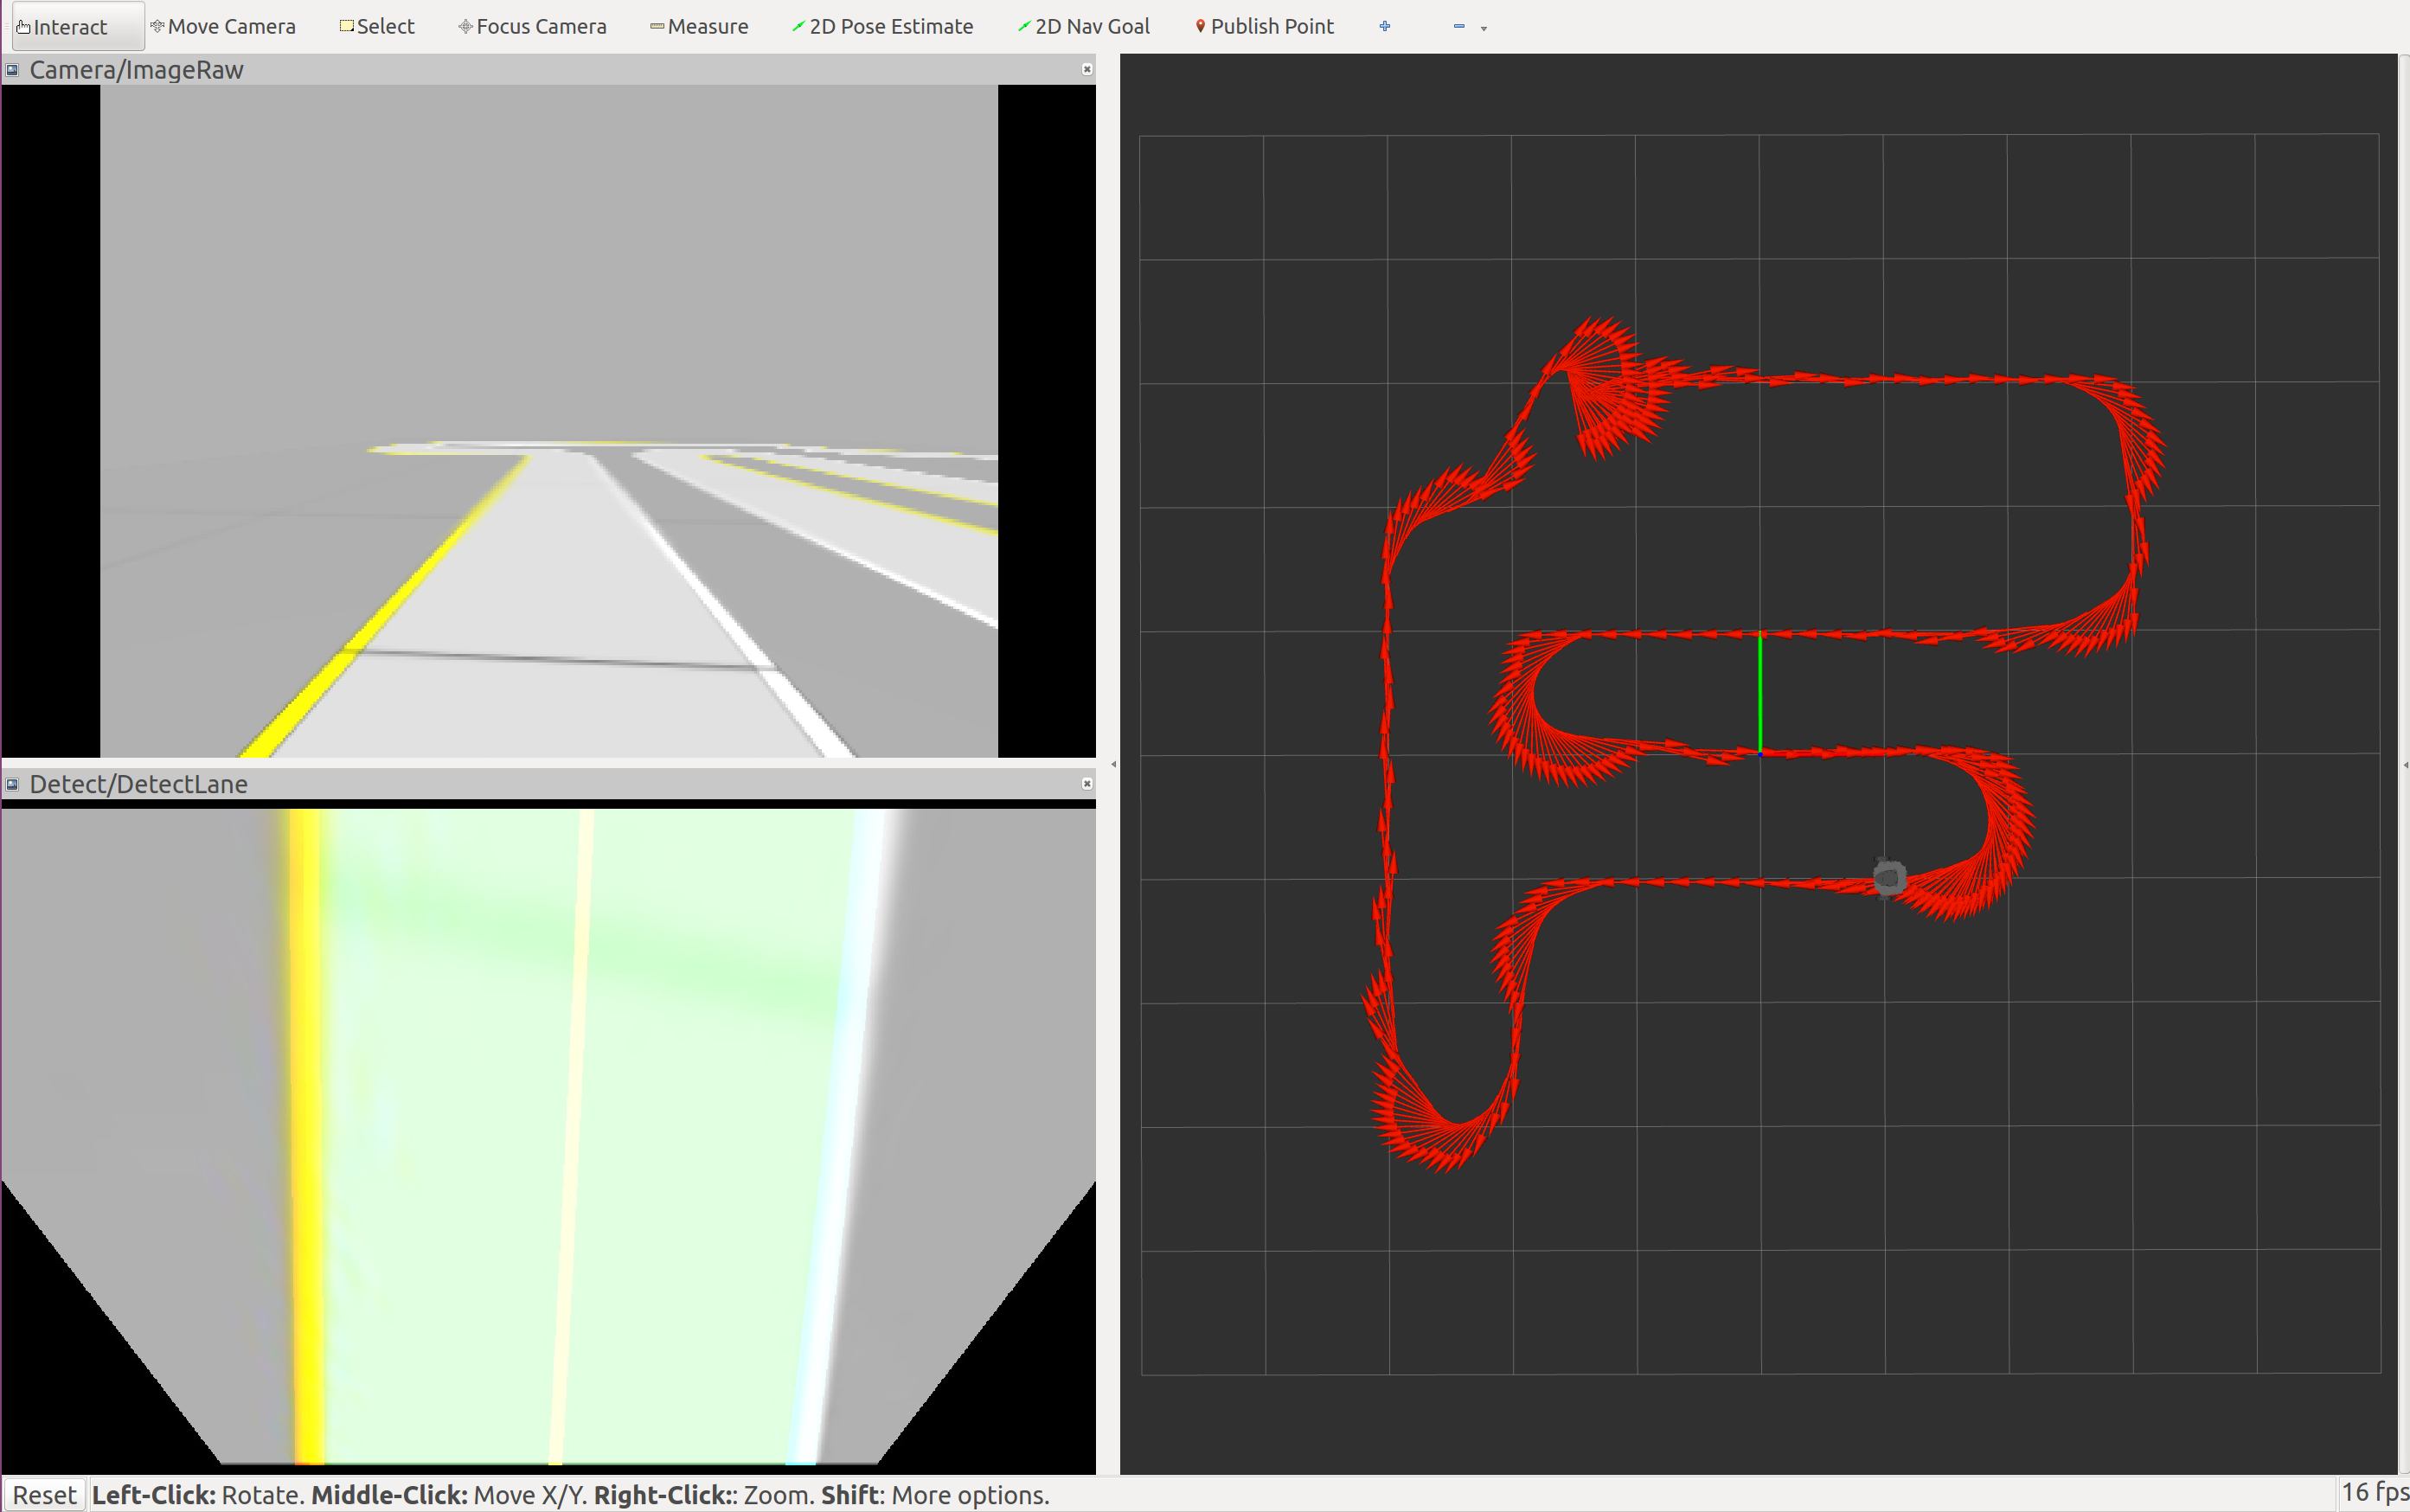
\includegraphics[width=0.65\textwidth]{figures/png/rviz}
\end{figure}

\end{frame}
